% =====================================================================================
% Starter manuscript. On the first Overleaf sync:
%   - blank Overleaf project      -> this file goes to Overleaf;
%   - Overleaf already has a draft -> the draft replaces this file (and references.bib).
%
% Journal class: replace the \documentclass line, for example
%   APS (PRA, PRL, ...): \documentclass[aps,pra,twocolumn,superscriptaddress,10pt]{revtex4-2}
%                        (put \maketitle after the abstract, use \affiliation, drop \date)
%   Elsevier:            \documentclass[preprint,12pt]{elsarticle}
%   Springer Nature:     use the sn-jnl template from the journal's Overleaf page
% =====================================================================================
\documentclass[11pt]{article}

\usepackage[margin=2.5cm]{geometry}
\usepackage{graphicx}
\usepackage{amsmath,amssymb}
\usepackage{bm}
\usepackage{booktabs}
\usepackage{array}
\newcolumntype{L}[1]{>{\raggedright\arraybackslash}p{#1}}
\usepackage{xcolor}
\usepackage[numbers,sort&compress]{natbib}
\usepackage{hyperref}

\hypersetup{colorlinks=true, linkcolor=blue!50!black, citecolor=blue!50!black, urlcolor=blue!50!black}
\graphicspath{{figures/}}              % figures written by run/*.py land in paper/figures/
\setlength{\emergencystretch}{2em}  % lets lines with long \texttt names break without overflowing

% Working notes: \showtodostrue -> \showtodosfalse hides every \TODO
\newif\ifshowtodos \showtodostrue
\newcommand{\TODO}[1]{\ifshowtodos\textcolor{red}{\textbf{[TODO:} #1\textbf{]}}\fi}
% Placeholder for a number that will come from data/experimentos/ (never type a result by hand)
\newcommand{\RES}[1]{\textcolor{orange!80!black}{\textbf{[#1]}}}
\newcommand{\ket}[1]{\lvert #1 \rangle}
\newcommand{\bra}[1]{\langle #1 \rvert}
\newcommand{\expval}[1]{\langle #1 \rangle}

\title{Qubit and continuous-variable quantum agents versus classical neural networks in Pong and Snake\TODO{final title}}
\author{Gubio G. de Lima\thanks{\TODO{affiliation}. E-mail: \texttt{gubio.gomes@estudante.ufscar.br}}}
\date{\today}

\begin{document}
\maketitle

\begin{abstract}
% DRAFT. Orange [brackets] = numbers that will come from data/experimentos/.
We compare three kinds of function approximators as deep Q-learning agents in two simple games
with a few discrete commands: Pong (stay, up, down) and Snake (up, down, left, right).
The agents are a discrete-variable variational quantum circuit (VQC) on qubits, a continuous-variable
quantum neural network (CV QNN) with Kerr non-linearities on optical modes, a Gaussian-only CV network
as an ablation, and classical multilayer perceptrons, one of them with the same number of trainable
parameters as the VQC.
All models are defined with PennyLane~\cite{bergholm2018pennylane} and trained by the same Double DQN code, the same
budget of environment steps and \RES{10} random seeds.
The game states are low dimensional (6 numbers in Pong, 8 in Snake), so each number is
encoded in one qubit, or two numbers in one optical mode, and the agents are fully quantum except for a
linear output scale. The CV network is simulated in the Fock basis by \texttt{cvjax}, a small JAX library
we wrote because PennyLane no longer has a working Fock device for this template.
\TODO{Main result in one sentence per game, with mean $\pm$ CI. Cost: time per step.}
Code, environments and data are open.
\end{abstract}

% =====================================================================================
\section{Introduction}\label{sec:intro}

Reinforcement learning (RL) agents learn by trial and error, and in deep RL a neural network
approximates the value of each action~\cite{mnih2013atari,mnih2015dqn}.
Variational quantum circuits---parametrized circuits trained by a classical
optimizer~\cite{cerezo2021vqa}---can take the place of that network.
They have been used as Q-functions and policies in standard benchmarks such as CartPole and
FrozenLake~\cite{chen2020vqc,lockwood2020rlqvc,skolik2022gym,jerbi2021pqp}, often reaching
classical performance with fewer parameters, although results depend strongly on the
baseline and the random seed~\cite{franz2022instab,meyer2022survey}.

Games are a natural next test. Atari Pong has been attempted with hybrid agents in which a
classical network compresses the screen pixels before a small circuit:
the first attempt did not learn~\cite{lockwood2021atari}, a later model matched the classical
score~\cite{freinberger2024atari}, and entangling circuits outperformed separable ones of the
same size in a competitive Pong setting~\cite{wang2026entanglement}.
In these works the classical encoder does much of the work, which makes it hard to tell what
the quantum part contributes. Continuous-variable (photonic) agents, the other main model of
quantum computation~\cite{killoran2019cvqnn,weedbrook2012gaussian}, have been tested on
CartPole~\cite{nagy2021photonic} and in latent observation spaces next to qubit
agents~\cite{nagy2024latent}, but not, to our knowledge, in games.
We also found no work on quantum agents in Snake.

\paragraph{Contributions.}
\begin{enumerate}
  \item Two open game environments, Pong and Snake, with small state vectors and 3--4 discrete
        actions, playable by humans and usable by agents (Sec.~\ref{sec:setup}).
  \item A like-for-like comparison of a qubit VQC, a CV QNN with Kerr gates, a Gaussian CV ablation and
        classical MLPs, all trained by one shared DQN implementation, with parameter-matched baselines
        and multiple seeds (Secs.~\ref{sec:setup} and~\ref{sec:training}).
  \item \texttt{cvjax}, an open JAX implementation of PennyLane's \texttt{CVNeuralNetLayers} in the Fock
        basis with exact gate matrix elements, verified against PennyLane and The Walrus
        (Supplementary Sec.~\ref{supp:cv}).
\end{enumerate}

Note on terms: ``quantum games'' usually means games about quantum physics or game theory
with quantum strategies~\cite{meyer1999strategies,eisert1999games,piispanen2023history,piispanen2022defining}.
Here the games are classical and only the agents are quantum.

% =====================================================================================
\section{Related work}\label{sec:related}

\paragraph{Variational quantum reinforcement learning.}
Chen~\textit{et al.}~\cite{chen2020vqc} introduced experience replay and target networks for
VQC Q-functions. Skolik~\textit{et al.}~\cite{skolik2022gym} showed that data re-uploading
and trainable input and output scaling are key for Q-learning with circuits, and
Jerbi~\textit{et al.}~\cite{jerbi2021pqp} did the same for policy gradients and proved a
learning separation for specially constructed tasks. Recurrent~\cite{chen2023qrnn},
evolutionary~\cite{chen2022evo} and policy-gradient~\cite{sequeira2023pg} variants followed;
\cite{meyer2022survey} reviews the field.

\paragraph{Games.}
\TODO{Expand: \cite{lockwood2021atari,freinberger2024atari,wang2026entanglement} (Pong from pixels),
\cite{maze2023hqnn,chen2022evo} (grid worlds, closest to Snake), classical Snake agents~\cite{wei2018snake}.}

\paragraph{Continuous variables.}
Killoran~\textit{et al.}~\cite{killoran2019cvqnn} mapped a neural-network layer to Gaussian
gates (affine part) followed by a non-Gaussian Kerr gate (activation).
Our single-mode regression study~\cite{delima2026regression} used this layer to fit functions and found
large gains for smooth targets but not for discontinuous ones.
\TODO{\cite{nagy2021photonic,nagy2024latent}: photonic PPO agents, comparison with qubits.}

\paragraph{Fair comparisons.}
Parameter-matched baselines~\cite{lockwood2020rlqvc}, many seeds and reporting of
variance~\cite{franz2022instab}, and the warning that hyperparameters matter more than parameter
count~\cite{skolik2022gym} shape our protocol.

% =====================================================================================
\section{Games and agents}\label{sec:setup}

\paragraph{Games.} Pong and Snake (Fig.~\ref{fig:games}) were written for this study in pure Python.
They can be played by a person and, through the same code, by an agent. The agent does not see the
screen: it receives a short list of numbers describing the game, six in Pong (ball position and
velocity, the two paddles) and eight in Snake (direction of the food, danger around the head, current
heading), and answers with one of a few commands: stay, up or down in Pong; up, down, left or right in
Snake. Scoring a point or eating gives a positive reward and losing a point or dying a negative one.
Settings and reference scores of simple rule-based players are in Supplementary Sec.~\ref{supp:envs}.

\begin{figure}[t]
  \centering
  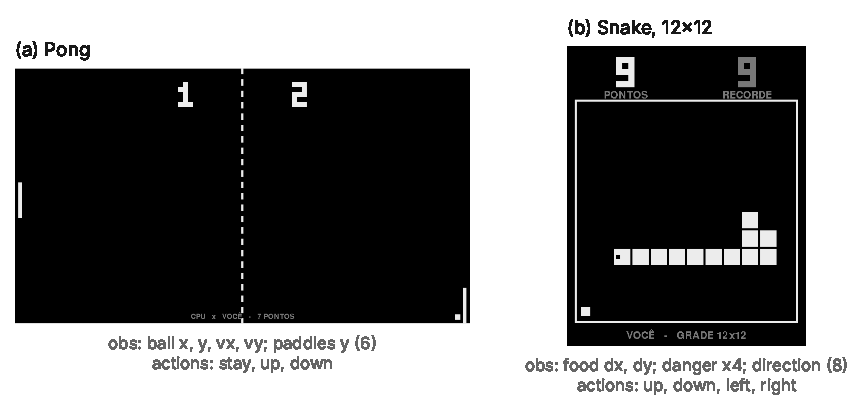
\includegraphics[width=\linewidth]{fig_jogos.pdf}
  \caption{The two games. Agents see only the short state vector described below each panel and send
  back one command per frame.}
  \label{fig:games}
\end{figure}

\paragraph{Agents.} Every agent answers the same question: given the game state, how good is each
command? It returns one number per command, its estimate of the future reward, and the agent plays the
command with the largest number. What changes is the model that computes these numbers:
\begin{itemize}
  \item \textbf{Qubit circuit (discrete variables).} Each number of the game state sets the rotation angle
        of one qubit; trainable rotations and entangling gates are interleaved with the data, which is
        written again in every layer~\cite{skolik2022gym,perezsalinas2020reuploading}. Measuring pairs of
        qubits gives one value per command (Fig.~\ref{fig:circuits}a).
  \item \textbf{Photonic network (continuous variables).} Pairs of numbers displace modes of light from the
        vacuum. Interferometers, squeezers and displacements mix and stretch the modes (the linear part of a
        neural layer), and Kerr gates make the response non-linear (the activation)~\cite{killoran2019cvqnn}.
        The average position quadrature of each mode gives one value per command (Fig.~\ref{fig:circuits}b).
        This is the architecture of our earlier regression study~\cite{delima2026regression}, extended to
        several modes. To see what the non-linearity adds, we also train a Gaussian version without Kerr gates.
  \item \textbf{Classical networks.} A standard multilayer perceptron, and a small one with as many trainable
        parameters as the qubit circuit, which is the fair point of comparison.
\end{itemize}
All quantum models are simulated on a classical computer. Architectures, sizes, initialization and the
simulators, including the \texttt{cvjax} library we wrote for the photonic network, are in Supplementary
Secs.~\ref{supp:models} and~\ref{supp:cv}.

\begin{figure}[t]
  \centering
  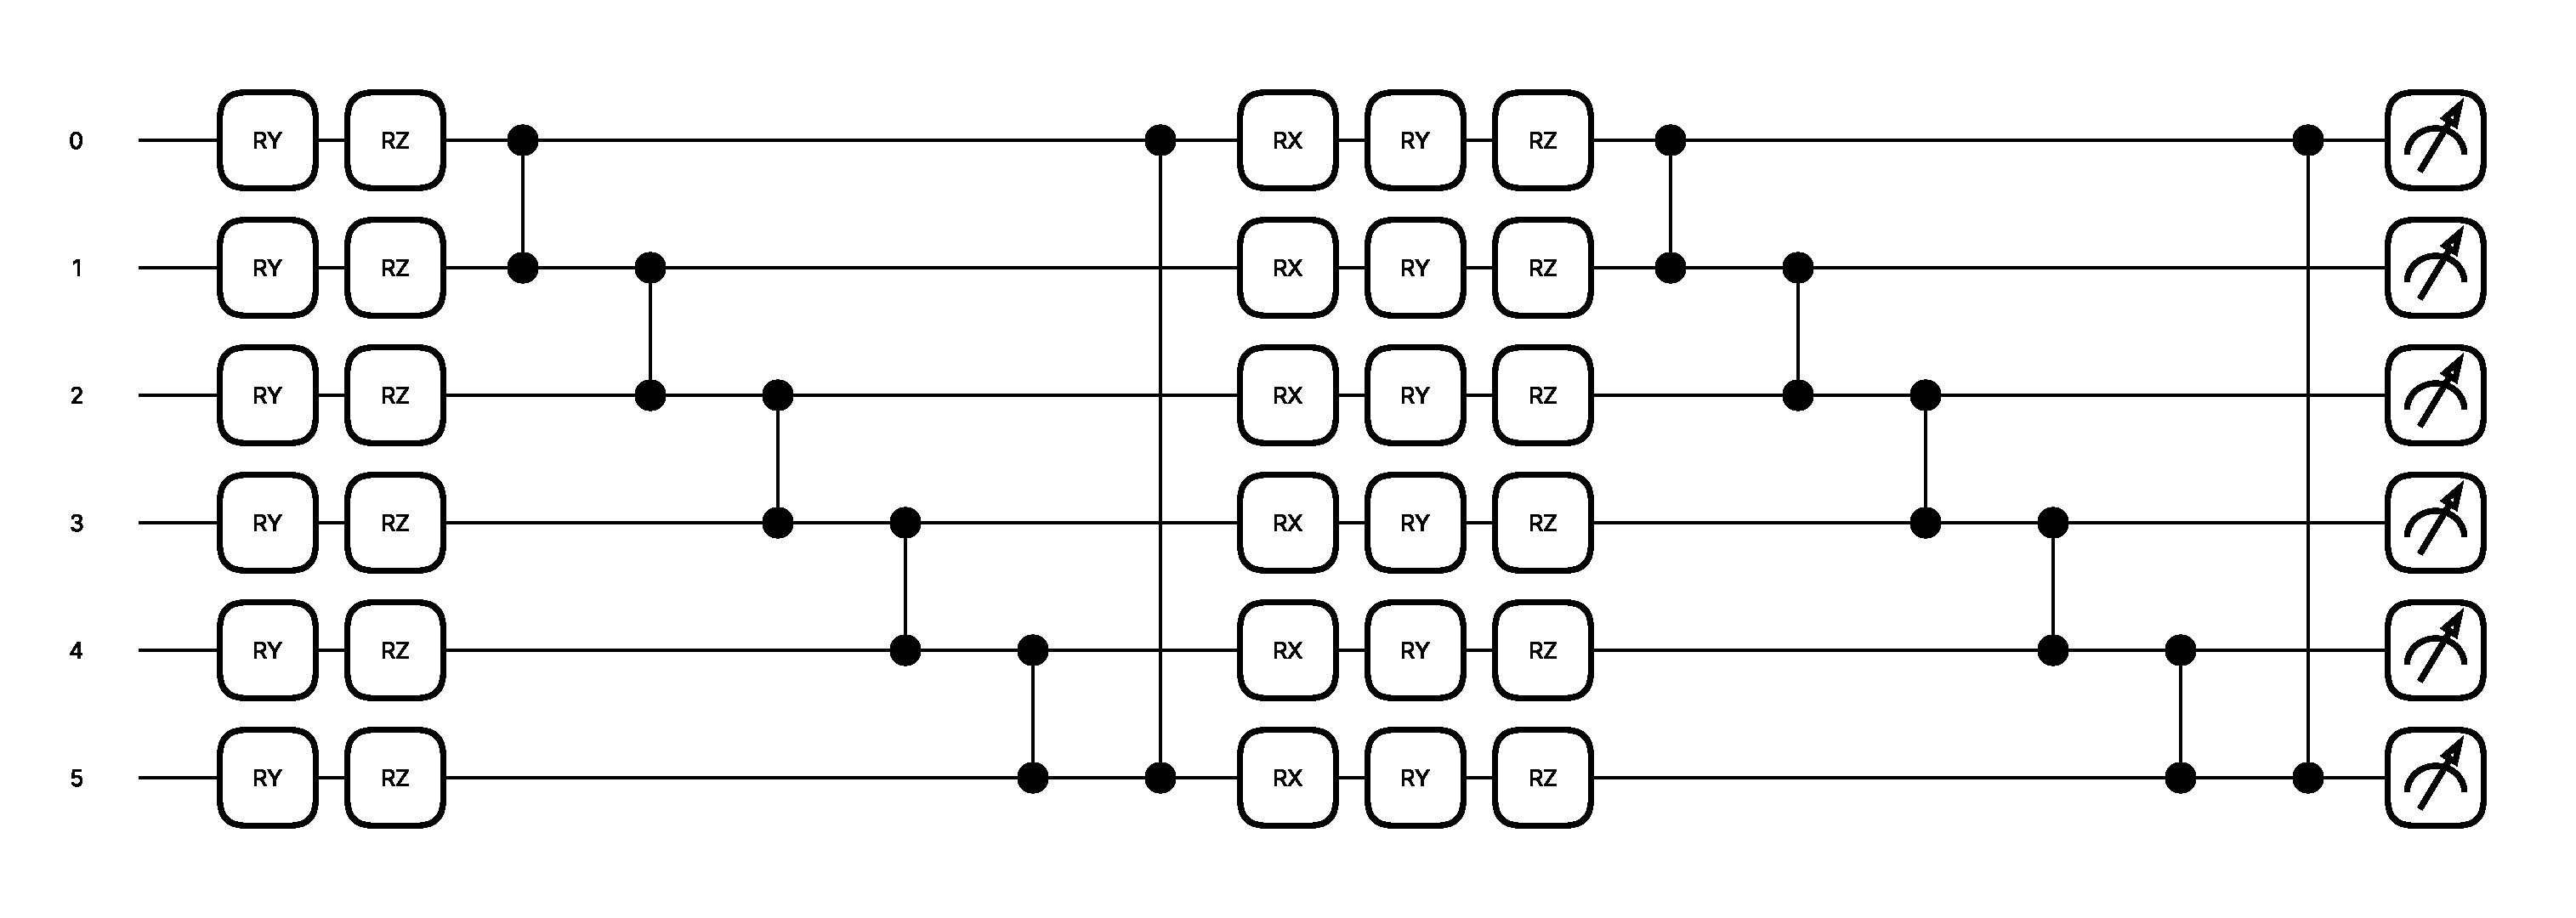
\includegraphics[width=\linewidth]{fig_circuito_qubits.pdf}\\[2pt]
  {\small (a) qubit circuit: one layer for Pong}\\[6pt]
  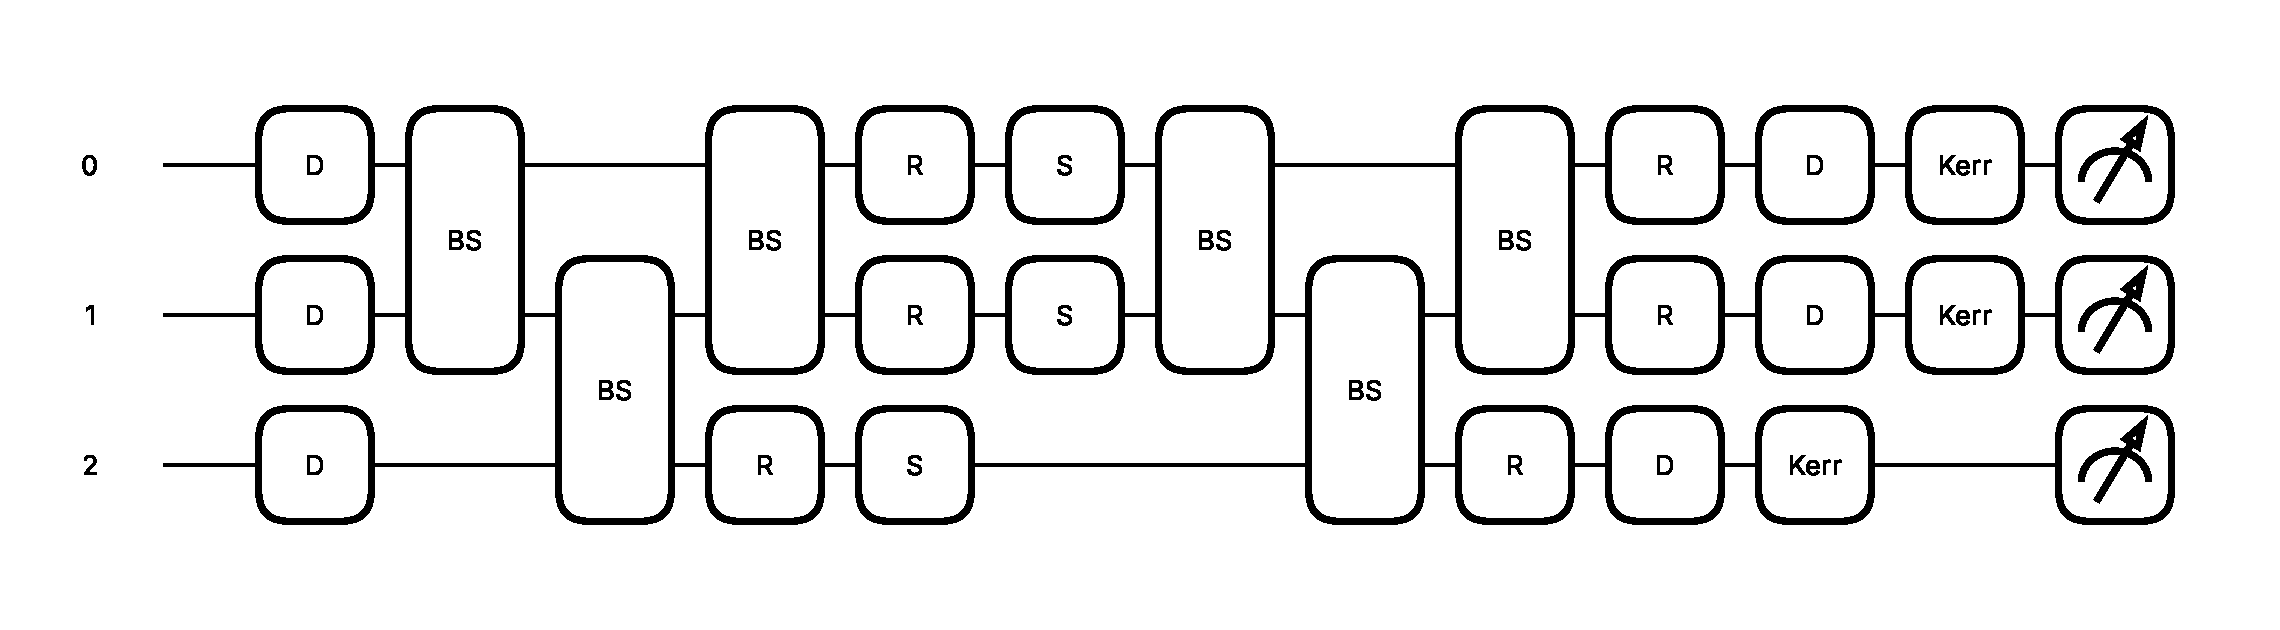
\includegraphics[width=\linewidth]{fig_circuito_cv.pdf}\\[2pt]
  {\small (b) photonic network: data encoding $D$ and one layer for Pong (BS beamsplitter, R rotation, S squeezing,
  D displacement, Kerr)}
  \caption{The two quantum models, drawn by PennyLane~\cite{bergholm2018pennylane} from the operations the
  agents execute. Each measurement on the right gives the value of one command.}
  \label{fig:circuits}
\end{figure}

% =====================================================================================
\section{Training}\label{sec:training}

The agents learn by playing, with deep Q-learning~\cite{mnih2015dqn,vanhasselt2016double}
(Fig.~\ref{fig:pipeline}). The same training code is used for every agent; only the model that turns a
game state into the values of the commands is swapped. This is what makes the comparison fair.

\begin{figure}[t]
  \centering
  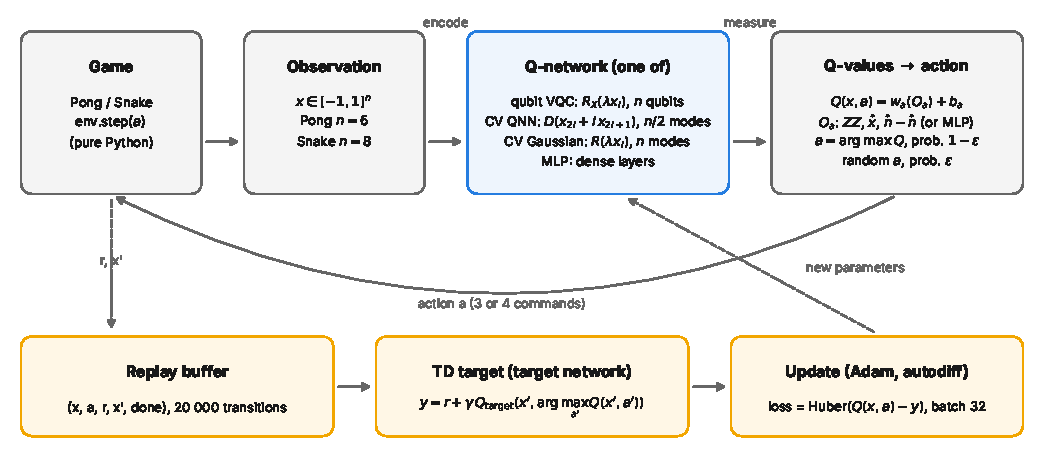
\includegraphics[width=\linewidth]{fig_fluxo.pdf}
  \caption{Training loop. The game sends its state, the model (quantum or classical) estimates the value of
  each command, and the agent plays the best one or, sometimes, a random one. Every move is stored; small
  random samples of past moves are used to correct the model, comparing its estimate with the reward
  obtained plus the value of what came next.}
  \label{fig:pipeline}
\end{figure}

One training run is one agent, one game and one random seed, and repeats four steps:
\begin{enumerate}
  \item \textbf{Play.} The agent plays the command its model values most. Early in training it often
        plays at random instead, to explore; this happens less and less as training goes on.
  \item \textbf{Remember.} The move, the reward and the next state are stored in a memory of recent moves.
  \item \textbf{Learn.} A small random sample of stored moves is replayed. For each one the model's estimate
        is compared with a target, the reward received plus the discounted value of the next state, and the
        parameters are moved to reduce the difference. For the quantum models this means changing gate
        angles, squeezing, displacement and Kerr strengths, using exact gradients of the simulated circuit.
  \item \textbf{Stabilize.} The target is computed with a slowly updated copy of the model, so the model does
        not chase its own changing estimates.
\end{enumerate}
At regular intervals the agent plays fresh games without exploration, and this score measures what it has
learned. Each agent is trained with several seeds, and we compare agents by the mean score and its
confidence interval. Hyperparameters, the exact update rule and the statistical protocol are in
Supplementary Secs.~\ref{supp:dqn} and~\ref{supp:stats}.

% =====================================================================================
\section{Results}\label{sec:results}

\textbf{Draft. The learning curves (Fig.~\ref{fig:curves}) and final scores (Fig.~\ref{fig:params}) shown
here are synthetic and only illustrate the planned figures; they are not results.}
They will be regenerated from \texttt{data/experimentos/} once the runs are complete. The cost
(Fig.~\ref{fig:cost}) is measured.

\paragraph{Learning.} \TODO{Qualitative description to write from the real curves. Points to address:
(i) do all agents learn to beat the random player in both games, and how early; (ii) at equal size, is the
qubit circuit ahead of, level with or behind the small classical network; (iii) does the photonic network
with Kerr gates learn more than its Gaussian version; (iv) how much do the curves vary between seeds;
(v) does the picture change from Pong (smooth motion, 3 commands) to Snake (grid, 4 commands)?}

\begin{figure}[t]
  \centering
  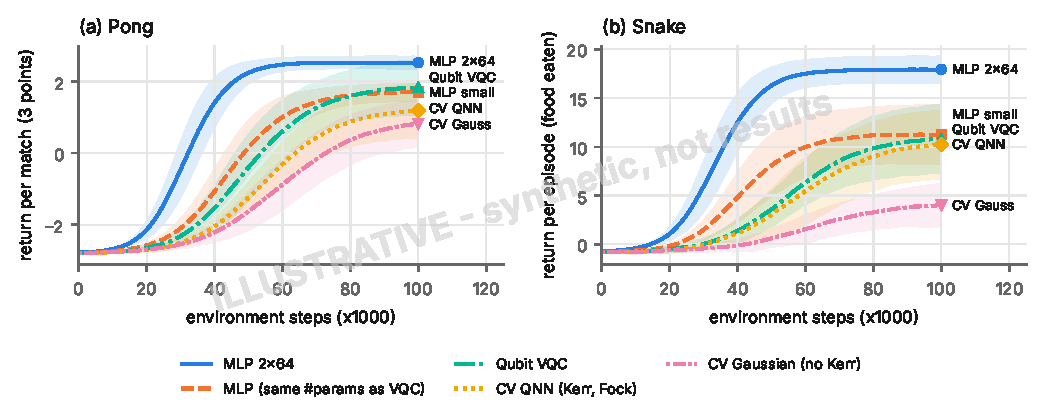
\includegraphics[width=\linewidth]{fig_curvas_ilustrativa.pdf}
  \caption{\textbf{Illustrative, synthetic data.} Planned figure: learning curves (mean $\pm$ standard deviation
  over seeds) of the five agents in Pong (a) and Snake (b). The shapes only reflect what earlier
  studies suggest~\cite{skolik2022gym,franz2022instab,nagy2021photonic}: small quantum models close to a
  classical model of the same size, with a larger spread between seeds.}
  \label{fig:curves}
\end{figure}

\paragraph{Size.} \TODO{Describe Fig.~\ref{fig:params}: final score against number of trainable
parameters. The comparison that matters is at equal size (quantum models versus the small classical network);
the large classical network shows what is reachable with many parameters.}

\begin{figure}[t]
  \centering
  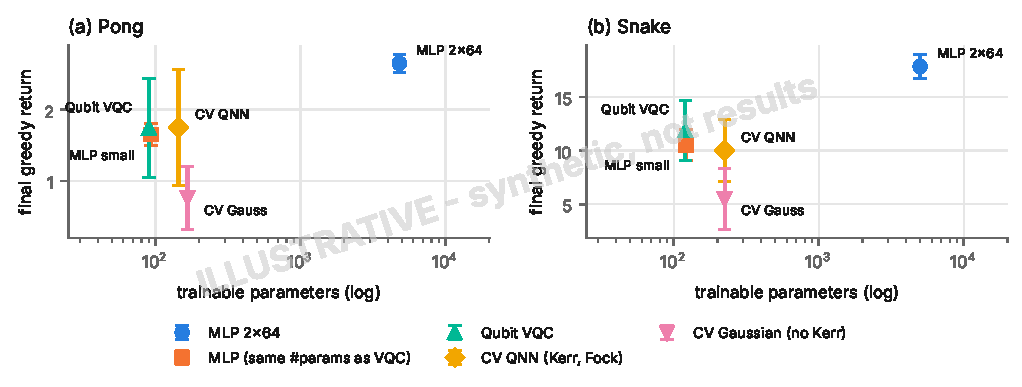
\includegraphics[width=\linewidth]{fig_parametros_ilustrativa.pdf}
  \caption{\textbf{Illustrative, synthetic data.} Planned figure: final score of the greedy policy (mean $\pm$
  standard deviation over seeds) against the number of trainable parameters.}
  \label{fig:params}
\end{figure}

\paragraph{Cost.} Simulating the quantum models on an ordinary processor is much slower than evaluating
classical networks of the same size: one to two orders of magnitude per training step
(Fig.~\ref{fig:cost}). The photonic network with Kerr gates is the most expensive, because its state must be
stored photon number by photon number for every mode, and Snake, with one more mode than Pong, costs about
four times more. This cost is a property of classical simulation, not of the quantum models themselves.

\begin{figure}[t]
  \centering
  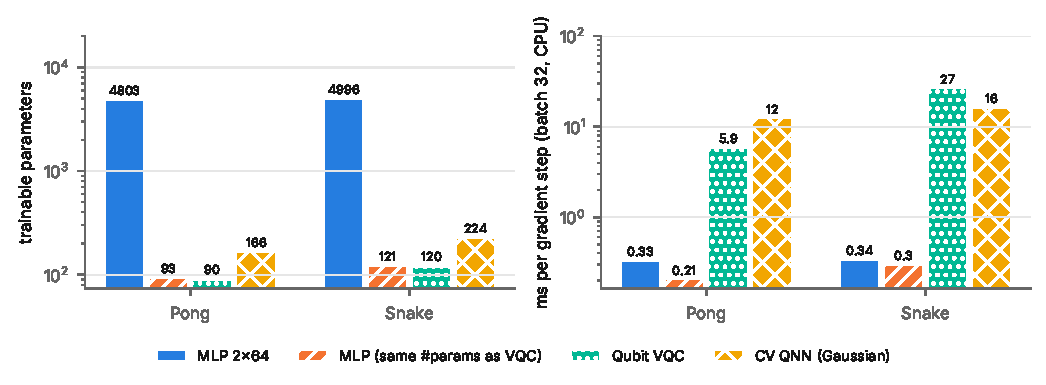
\includegraphics[width=\linewidth]{fig_custo.pdf}
  \caption{Measured cost of each agent: trainable parameters (left) and time per training step on a
  CPU simulator (right), log scales. Computer and exact values: Supplementary Sec.~\ref{supp:cost}.}
  \label{fig:cost}
\end{figure}

Planned ablations: entanglement (qubit circuit without CZ gates, as in~\cite{wang2026entanglement}),
depth (number of layers), and the Fock cutoff of the photonic network.

% =====================================================================================
\section{Discussion}\label{sec:discussion}
\TODO{After results. Points to cover: what ``comparable'' means given the confidence intervals; cost
on simulators versus hardware; the observations are hand-designed and low dimensional, so the
results say nothing about learning from pixels; no hardware noise; no claim of quantum advantage
(see~\cite{meyer2022survey}).}

\section{Conclusions}\label{sec:conclusions}
\TODO{}

\paragraph{Code and data availability.}
Games, agents, training scripts and the data behind every figure and table:
\TODO{repository URL / Zenodo DOI}. The photonic simulator is available at
\url{https://github.com/GubioGL/cvjax}. Figures and Supplementary tables are regenerated by
\texttt{run/figuras\_artigo.py} and \texttt{run/tabelas\_suplementares.py}.

\bibliographystyle{unsrtnat}
\bibliography{references}

% =====================================================================================
% SUPPLEMENTARY MATERIAL: every technical detail. Tables in supp/ are generated by
% run/tabelas_suplementares.py and tab_custo.tex by run/figuras_artigo.py: do not edit them by hand.
% =====================================================================================
\clearpage
\appendix
\renewcommand{\thesection}{S\arabic{section}}
\renewcommand{\thetable}{S\arabic{table}}
\renewcommand{\thefigure}{S\arabic{figure}}
\renewcommand{\theequation}{S\arabic{equation}}
\setcounter{table}{0}\setcounter{figure}{0}\setcounter{equation}{0}
\begin{center}{\Large\bfseries Supplementary Material}\end{center}

\section{Computational setup}\label{supp:machine}
All simulations run on CPU, in single precision (complex64/float32), with JAX~\cite{jax2018github} just-in-time
compilation. Table~\ref{tab:machine} lists the computer and software on which the costs of
Sec.~\ref{supp:cost} were measured (\texttt{data/custo/maquina.json}).
\TODO{If the training runs are done on another computer, rerun \texttt{run/medir\_custo.py} there.}

\begin{table}[h]
  \centering
  \caption{Computer and software of the measurements.}
  \label{tab:machine}
  % generated by run/tabelas_suplementares.py -- do not edit by hand
\begin{tabular}{ll}
\toprule
CPU & Intel(R) Xeon(R) Processor @ 2.10GHz \\
logical cores & 4 \\
RAM & 15.7 GB \\
GPU & none (all simulations on CPU) \\
operating system & Ubuntu 24.04.5 LTS (Linux 6.18.44-fc-v880) \\
Python & 3.13.18 \\
jax & 0.7.1 \\
jaxlib & 0.7.1 \\
pennylane & 0.45.1 \\
optax & 0.2.9 \\
numpy & 2.5.3 \\
pygame & 2.6.1 \\
cvjax & 0.1.0 \\
\bottomrule
\end{tabular}

\end{table}

\section{Games}\label{supp:envs}
Both games are deterministic for a given seed and follow the \texttt{reset}/\texttt{step} interface of
Gymnasium~\cite{towers2024gymnasium}. All observations are scaled to $[-1,1]$. Episodes cut by a time limit
are treated as truncated, not terminal (their value is still bootstrapped). Table~\ref{tab:envs} gives the
settings used in training, read from the code; Table~\ref{tab:reference} the scores of simple players over
30 episodes with seeds not used for training (\texttt{data/referencia/baselines.csv}).

\begin{table}[h]
  \centering
  \caption{Game settings used in the experiments.}
  \label{tab:envs}
  % generated by run/tabelas_suplementares.py -- do not edit by hand
\small
\begin{tabular}{L{2.5cm}L{6.2cm}L{6.2cm}}
\toprule
 & Pong & Snake \\
\midrule
field / grid & 1280$\times$720 px & 12$\times$12 cells \\
observation & ball $x,y,v_x,v_y$; player, CPU paddle $y$ (6) & food $\Delta x,\Delta y$; danger up/down/left/right; heading $d_x,d_y$ (8) \\
actions & stay, up, down (3) & up, down, left, right (4); reversing is ignored \\
reward & $+1$ point won, $-1$ point lost, $+0.1$ per return & $+1$ food, $-1$ death, $-0.01$ per step \\
episode end & first to 3 points, or 5000 steps (truncation) & death, or 200 steps without food / 5000 steps (truncation) \\
paddle / ball & paddle 10$\times$100 px, ball 15 px & start length 3 \\
speeds (px/step) & player 9.0, CPU 6.0, ball 7.0$\to$14.0 ($\times1.06$ per hit) & 1 cell per step \\
bounce & angle up to 60$^\circ$ depending on hit position & --- \\
opponent & rule-based CPU paddle, reacts after 50\% of the width & --- \\
frame rate & 1 step = 1 frame at 60 FPS & 1 step = 1 move \\
\bottomrule
\end{tabular}

\end{table}

\begin{table}[h]
  \centering
  \caption{Reference scores: rule-based players (Pong: paddle follows the ball; Snake: greedy walk to the
  food avoiding immediate danger) and random actions, 30 episodes each.}
  \label{tab:reference}
  % generated by run/tabelas_suplementares.py -- do not edit by hand
\begin{tabular}{llrr}
\toprule
game & policy & return (mean $\pm$ sd) & points / food \\
\midrule
Pong & rule-based & $2.71\pm1.03$ & 1.1 \\
Pong & random & $-2.94\pm0.07$ & 0.0 \\
Snake & rule-based & $18.32\pm6.41$ & 21.1 \\
Snake & random & $-1.09\pm0.33$ & 0.1 \\
\bottomrule
\end{tabular}

\end{table}

\section{Models}\label{supp:models}
Every model maps $\bm{x}\in[-1,1]^n$ ($n=6$ Pong, 8 Snake) to $Q(\bm x,a)$, one value per action. Quantum
models read one observable per action and rescale it with trainable $w_a,b_a$, because expectation values are
bounded while returns are not. Table~\ref{tab:models} lists architecture, register, initialization,
learning rates and parameter counts.

\begin{table}[h]
  \centering
  \caption{Models ($L$ = layers). Parameter counts include the output scales $w,b$ and input scales.}
  \label{tab:models}
  % generated by run/tabelas_suplementares.py -- do not edit by hand
\small
\setlength{\tabcolsep}{4pt}
\begin{tabular}{L{1.9cm}L{4.1cm}L{1.9cm}L{3.3cm}L{1.6cm}rr}
\toprule
agent & architecture & register & initialization & learning rate & \multicolumn{2}{c}{parameters} \\
 & & (Pong / Snake) & & & Pong & Snake \\
\midrule
MLP $2\times64$ & dense ReLU layers 64$\times$64 & --- & He-uniform weights, zero biases & $10^{-3}$ (all) & 4803 & 4996 \\
MLP, VQC-matched & one ReLU layer of width 9 (parameters $\approx$ VQC) & --- & He-uniform weights, zero biases & $10^{-3}$ (all) & 93 & 121 \\
qubit VQC & $L=4$ re-uploading layers: $R_YR_Z$ + CZ ring, $R_X(\lambda x_i)$; read-out $w_a\langle Z_{2a}Z_{2a+1}\rangle+b_a$ & 6 / 8 qubits & $\theta\sim U(0,2\pi)$, $\lambda=\pi/2$, $w=1$, $b=0$ & $10^{-3}$; $w,b$: $10^{-2}$ & 90 & 120 \\
CV QNN (Kerr) & encoding $D(s x_{2i}+i s x_{2i+1})$ once; $L=4$ \texttt{CVNeuralNetLayers} layers; read-out $w_a\langle\hat x_a\rangle+b_a$ & 3 / 4 modes, Fock cutoff 6 & active ($r,a,k$) $\sim\mathcal N(0,10^{-4})$, passive $\sim\mathcal N(0,0.1)$, $s=0.5$, $w=1$, $b=0$ & $10^{-3}$; $w,b$: $10^{-2}$ & 144 & 224 \\
CV Gaussian & $L=4$ layers: $S$, $D$, $R(\lambda x_i)$, beamsplitter chain; read-out $w_a(\langle\hat n_{2a}\rangle-\langle\hat n_{2a+1}\rangle)+b_a$ & 6 / 8 modes (Gaussian) & $r\sim U(0,0.1)$, $|d|=0.5$, phases $\sim U(0,2\pi)$, $\lambda=\pi/2$, $w=1$, $b=0$ & $10^{-3}$; $w,b$: $10^{-2}$ & 166 & 224 \\
\bottomrule
\end{tabular}

\end{table}

\paragraph{Qubit circuit.} With one qubit per observation component,
\begin{equation}
  \ket{\psi(\bm{x})} = W(\bm\theta_L)\prod_{\ell=0}^{L-1} S(\bm\lambda_\ell \odot \bm{x})\, W(\bm\theta_\ell)\,\ket{0}^{\otimes n},
  \qquad S(\bm{z}) = \bigotimes_i R_X(z_i),
\end{equation}
where $W(\bm\theta)$ applies $R_Y R_Z$ to every qubit followed by a ring of CZ gates. The input scales start at
$\lambda=\pi/2$, so $x\in[-1,1]$ maps to $[-\pi/2,\pi/2]$ ($\pm\pi$ would be the same rotation up to a global
phase). Read-out: $Q(\bm{x},a) = w_a \expval{Z_{2a} Z_{2a+1}} + b_a$. Simulator: PennyLane
\texttt{default.qubit}, backpropagation through JAX.

\paragraph{Photonic network with Kerr gates.} With $M=n/2$ modes (3 in Pong, 4 in Snake), the input is
$\ket{\psi_0(\bm x)}=\bigotimes_{i} D(\alpha_i)\ket{0}$, $\alpha_i=s_{2i}x_{2i}+i\,s_{2i+1}x_{2i+1}$, applied once.
Each of the $L$ layers is PennyLane's \texttt{CVNeuralNetLayers}~\cite{killoran2019cvqnn}:
\begin{equation}
  \mathcal L = \prod_i K(k_i)\,\prod_i D(a_i e^{i\phi_{a,i}})\; U_2(\bm\theta_2,\bm\phi_2,\bm\varphi_2)\,\prod_i S(r_i,\phi_{r,i})\; U_1(\bm\theta_1,\bm\phi_1,\bm\varphi_1),
\end{equation}
with interferometers $U_{1,2}$ (rectangular mesh of $M(M-1)/2$ beamsplitters and $M$ rotations), squeezing $S$,
displacement $D$ and Kerr $K(k)=e^{ik\hat n^2}$. Read-out:
$Q(\bm{x},a) = w_a\,\bra{\psi_L}\hat x_a\ket{\psi_L} + b_a$, $\hat x=\sqrt{\hbar/2}(\hat a+\hat a^\dagger)$, $\hbar=2$.
For one mode the interferometers reduce to rotations and a layer is $R\,S\,R\,D\,K$, the regression network
of~\cite{delima2026regression}. The input is not re-uploaded because successive displacements add up, raising
the photon number above the cutoff; active parameters start at $\mathcal N(0,10^{-4})$ as in the PennyLane
demo~\cite{pennylane_cvqnn_demo}.

\paragraph{Gaussian photonic network (ablation).} One mode per observation component; each layer applies
$S(r_i,\phi_i)$ and $D(d_i,\psi_i)$ to every mode, the data as phase rotations $R(\lambda_i x_i)$ (which add no
photons and are re-uploaded), and a beamsplitter chain. Read-out
$Q(\bm{x},a) = w_a(\expval{\hat n_{2a}}-\expval{\hat n_{2a+1}})+b_a$. Gaussian states are described by a mean vector
$\bm\mu$ and covariance matrix $V$~\cite{weedbrook2012gaussian}; a gate with symplectic matrix $M_g$ maps
$\bm\mu\to M_g\bm\mu$, $V\to M_gVM_g^{\mathsf T}$, and
$\expval{\hat n_i}=(V_{x_ix_i}+V_{p_ip_i}+\mu_{x_i}^2+\mu_{p_i}^2)/(2\hbar)-1/2$.

\paragraph{Classical networks.} ReLU MLPs: $2\times64$, and one hidden layer whose width matches the parameter
count of the qubit circuit.

\section{Simulation of the photonic network (cvjax)}\label{supp:cv}
The Kerr gate makes the state non-Gaussian, so it is stored as $D_c^M$ amplitudes in the Fock basis with
$D_c=6$ photons per mode (216 amplitudes in Pong, 1296 in Snake). PennyLane's only Fock device for
\texttt{CVNeuralNetLayers}, \texttt{strawberryfields.fock}, requires PennyLane $<0.30$, and
\texttt{default.gaussian} does not accept Kerr gates. We therefore wrote \texttt{cvjax}
(\url{https://github.com/GubioGL/cvjax}), a small JAX library inspired by Strawberry Fields~\cite{killoran2019sf}
and by the CV-QuForge and QuIara simulators of T.~de~S.~Farias and A.~C.~Ricardo:
\begin{itemize}
  \item each gate acts on the tensor axis of its mode(s), without building the full $D_c^M\times D_c^M$ matrix;
  \item gate matrices are the exact elements of the untruncated operators below the cutoff: normal-ordered
        forms for displacement and squeezing, e.g.\ $D(\alpha)=e^{-|\alpha|^2/2}e^{\alpha\hat a^\dagger}e^{-\alpha^*\hat a}$
        (no intermediate state crosses the cutoff), and, for the beamsplitter, the full rotation within each block of
        fixed total photon number, cut afterwards;
  \item verification (unit tests): gates agree with The Walrus~\cite{gupt2019walrus} and with \texttt{expm} at
        cutoff 60 to $\sim10^{-7}$; layers reproduce the decomposition of \texttt{qml.CVNeuralNetLayers} gate by gate;
        with $k=0$, $\expval{\hat n}$ and $\expval{\hat x}$ agree with \texttt{default.gaussian} to $<2\times10^{-4}$.
\end{itemize}
Truncation is monitored by the leakage $1-\langle\psi_L|\psi_L\rangle$: $\lesssim1.4\times10^{-3}$ at initialization
for the most extreme inputs. \TODO{Report the maximum leakage after training.}
The Gaussian ablation is simulated exactly in JAX with the mean--covariance formalism and checked against
\texttt{default.gaussian} ($\sim10^{-7}$).

\section{Training algorithm and hyperparameters}\label{supp:dqn}
Double DQN~\cite{mnih2015dqn,vanhasselt2016double}, identical for all models (\texttt{src/rl/dqn.py}), with the
values of Table~\ref{tab:dqn}. At step $t$ the agent takes a random action with probability $\varepsilon_t$ and
$a_t=\arg\max_a Q_{\bm w}(\bm x_t,a)$ otherwise; the transition $(\bm x_t,a_t,r_t,\bm x_{t+1},d_t)$ enters the replay
buffer, with $d_t=1$ only for true terminal states. After each step a mini-batch $\mathcal B$ is sampled and
\begin{equation}
  y = r + \gamma(1-d)\,Q_{\bm w^-}\!\big(\bm x',\arg\max_{a'}Q_{\bm w}(\bm x',a')\big),\qquad
  \mathcal L(\bm w)=\frac1{|\mathcal B|}\sum_{\mathcal B}\mathrm{Huber}\big(Q_{\bm w}(\bm x,a)-y\big),
\end{equation}
with the target parameters $\bm w^-$ copied from $\bm w$ at fixed intervals. Each step evaluates the model
$3|\mathcal B|$ times (online at $\bm x$ and $\bm x'$, target at $\bm x'$). On the simulators gradients are exact
(automatic differentiation through the state vector, Fock tensor or covariance matrix); on hardware they would be
estimated by the parameter-shift rule. The output scale and bias of the quantum models use a larger learning
rate, following~\cite{skolik2022gym}. \TODO{Decide whether the MLPs' last layer should get the same rate.}

\begin{table}[h]
  \centering
  \caption{Training hyperparameters (\texttt{src/experimentos.py}); identical for all agents, and for both games
  except the learning rate.}
  \label{tab:dqn}
  % generated by run/tabelas_suplementares.py -- do not edit by hand
\begin{tabular}{ll}
\toprule
algorithm & Double DQN, Huber loss, Adam \\
environment steps per run & $100\,000$ \\
discount $\gamma$ & 0.99 \\
learning rate (circuit / MLP) & $10^{-3}$ \\
learning rate of $w,b$ (quantum output) & $10^{-2}$ \\
mini-batch & 32 \\
replay buffer & $20\,000$ \\
warm-up (random actions) & 1000 steps \\
gradient step & every 1 environment step(s) \\
target network update & every 500 gradient steps \\
$\varepsilon$-greedy & 1.0 $\to$ 0.05, linear over $40\,000$ steps \\
gradient clipping & global norm 10.0 \\
quantum layers $L$ & 4 \\
Fock cutoff (CV QNN) & 6 per mode \\
\bottomrule
\end{tabular}

\end{table}

\paragraph{Choice of the learning rate.} The shared settings were checked with the classical MLP, which is the
cheapest to train, using 3 seeds and the full budget of $10^5$ steps (Table~\ref{tab:tuning}; score = mean of the
last six greedy evaluations of each seed, data in \texttt{data/ajuste/}). In Pong the default learning rate
($10^{-3}$) gave unstable play, with the greedy score swinging between $-3$ and $+3$ during training, and
$3\times10^{-4}$ gave a clearly better and steadier result; a slower target network (update every 2000 steps)
learned too slowly within the budget. The other changes tried (batch size, target update every 250 steps) were
within the seed-to-seed noise, so only the learning rate was changed. In Snake the difference between
$10^{-3}$ and $3\times10^{-4}$ was within the noise, so the original value was kept. \textbf{This selection used only the
classical baseline and may favor it; the learning rates of the quantum models were not tuned.}
\TODO{Run the same small sweep for the quantum agents, with the same budget.}

\begin{table}[h]
  \centering
  \caption{Sweep of training settings with the MLP (score: mean over seeds of the last six greedy evaluations;
  individual seeds in parentheses; reference return: random $-2.94$, rule-based $+2.71$ in Pong; $-1.09$ and
  $+18.3$ in Snake).}
  \label{tab:tuning}
  % generated by run/tabelas_suplementares.py -- do not edit by hand
\small
\begin{tabular}{rrrL{4.3cm}L{4.3cm}}
\toprule
learning rate & target update & batch & Pong: mean (per seed) & Snake: mean (per seed) \\
\midrule
$10^{-3}$ & 500 & 32 & $-0.88$ ($0.1$, $-1.1$, $-1.6$) & $17.20$ ($17.9$, $16.2$, $17.5$) \\
$3\times10^{-4}$ & 500 & 64 & $0.82$ ($1.4$, $1.4$, $-0.3$) & --- \\
$3\times10^{-4}$ & 500 & 32 & $0.66$ ($-0.2$, $0.4$, $1.8$) & $16.28$ ($16.1$, $14.5$, $18.3$) \\
$3\times10^{-4}$ & 250 & 32 & $0.64$ ($0.7$, $0.4$, $0.9$) & --- \\
$10^{-4}$ & 500 & 32 & $0.03$ ($0.5$, $0.2$, $-0.6$) & --- \\
$3\times10^{-4}$ & 2000 & 32 & $-2.12$ ($-1.8$, $-2.4$, $-2.2$) & --- \\
$10^{-3}$ & 2000 & 32 & $-2.20$ ($-2.7$, $-2.1$, $-1.8$) & --- \\
\bottomrule
\end{tabular}

\end{table}

\section{Evaluation and statistics}\label{supp:stats}
Each agent is trained with \RES{10} seeds per game; a seed fixes the game, the initialization and the replay
sampling. Every \RES{5000} steps the greedy policy ($\varepsilon=0$) plays 5 episodes with seeds not used for
training. Learning curves store, per episode, return, length, $\varepsilon$, loss and wall time
(\texttt{data/experimentos/<game>/<agent>/seed\_<n>.csv}, settings in a JSON file next to each). We report means
with 95\% bootstrap confidence intervals and steps to reach a threshold (\RES{Pong: $+1$; Snake: 10 food}), and
compare each quantum model with the parameter-matched MLP with a Mann--Whitney test.

\section{Measured cost}\label{supp:cost}
Table~\ref{tab:cost} gives the values of Fig.~\ref{fig:cost}: time per training step (mini-batch of 32, steady
state after JIT compilation), measured by \texttt{run/medir\_custo.py} on the computer of Table~\ref{tab:machine}.

\begin{table}[h]
  \centering
  \caption{Trainable parameters and time per training step.}
  \label{tab:cost}
  % generated by run/figuras_artigo.py from data/custo/custo_por_agente.csv
\begin{tabular}{lrrrr}
\toprule
 & \multicolumn{2}{c}{parameters} & \multicolumn{2}{c}{ms / gradient step} \\
agent & Pong & Snake & Pong & Snake \\
\midrule
MLP $2\times64$ & 4803 & 4996 & 0.354 & 0.355 \\
MLP, VQC-matched & 93 & 121 & 0.276 & 0.268 \\
qubit VQC & 90 & 120 & 6.65 & 26.5 \\
CV QNN (Kerr, Fock) & 144 & 224 & 30.4 & 112 \\
CV Gaussian (no Kerr) & 166 & 224 & 11.4 & 18.1 \\
\bottomrule
\end{tabular}

\end{table}


\end{document}
